\documentclass[a4paper]{jpconf}
\usepackage{graphicx}
\usepackage{listings}
\usepackage{multirow}
\begin{document}
\title{Dirac integration with a general purpose bookkeeping DB: a complete general suite for distributed resources exploitation}

\author{M Chrzaszcz$^{1,2}$, C De Santis$^3$, G Donvito$^4$, A Fella$^{5,6}$, R Grzymkowski$^2$, B Santeramo$^{4,7}$, L Tomassetti$^{6,8}$, M Zdybal$^2$}
\address{$^1$ Physik-Institut, Universitat Zurich, Zurich, Switzerland}
\address{$^2$ Henryk Niewodniczanski Institute of Nuclear Physics Polish Academy of Sciences, Krakow, Poland}
\address{$^3$ INFN - Sezione di Roma Tor Vergata, Roma, Italy}
\address{$^4$ INFN - Sezione di Bari, Bari, Italy}
\address{$^5$ INFN - Sezione di Pisa, Pisa, Italy}
\address{$^6$ Dipartimento di Matematica e Informatica, Universit\'a di Ferrara, Ferrara, Italy}
\address{$^7$ Dipartimento Interateneo di Fisica dell’Universit\'a e del Politecnico di Bari, Bari, Italy}
\address{$^8$ INFN - Sezione di Ferrara, Ferrara, Italy}
\ead{bruno.santeramo@ba.infn.it}

\begin{abstract}
In the context of High Energy Physics computing field the R\&D studies aimed to
the definition of the data and workload models have been carried on and 
completed by the Super$B$ community beyond the experiment life itself.
The work resulted of great interest for a generic mid- and small size VO to 
fulfill Grid exploiting requirements involving CPU-intensive tasks.

We present the R\&D line achievements in the design, developments and test of a
distributed resource exploitation suite based on DIRAC. The main components of
such a suite are the information system, the job wrapper and the new generation
DIRAC framework. The DB schema and the SQL logic have been designed to be able
to be adaptive with respect to the VO requirements in terms of physics 
application, job environment and bookkeeping parameters. A deep and flexible 
integration with DIRAC features has been obtained using SQLAlchemy technology
allowing mapping and interaction with the information system. A new DIRAC
extension has been developed to include this functionality along with a new set
of DIRAC portal interfaces aimed to the job, distributed resources, and
metadata management. The results of the first functionality and efficiency
tests will be reported.
\end{abstract}

\section{Introduction}

In HEP as well in other fields, the necessity to manage and analyze huge amount of data or simulate large amount of events is a typical issue.
Today several solutions available for this purpose exist, but lot of them are developed for particular needs of a specific customer.
During Super$B$ R\&D activities, a solution useful for Super$B$ was deployed which can be easily adopted by a generic small and mid-size VO.

\section{Suite description}
% Marcin
%philosophy: simple, standard and long term solution\\
%bird's eye view all over the project\\

In order to develop a simple, standard and long term solution, suite components (adopted or developed) should be flexible enough to be adapted in order to fulfill needs of a generic VO.\\
Suite components include DIRAC\cite{ref:dirac}, the Information System and the Job Wrapper (see figure \ref{fig:project_bird_eye}).\\
\begin{itemize}
\item DIRAC is a well known and widely adopted framework to manage Grid resources, job submission, workflow definition, user authentication, authorization and accounting.
\item The Information System holds metadata related to simulations and information about dataset structures and data placement on Grid resources. Information System is a PostgreSQL\cite{ref:postgres} database. DIRAC interact with Information System via SQLAlchemy\cite{ref:sqlalchemy}.
\item The Job Wrapper, executed in bundle with jobs, updates Information System about simulations status and data placement using a REST interface. Job Wrapper is a python script.
\end{itemize}

\begin{figure}[h]
\includegraphics[width=26pc]{img/project_bird_eye_2.eps}\hspace{2pc}%
\caption{\label{fig:project_bird_eye}Project bird's eye view.}
\end{figure}

%\begin{figure}[h]
%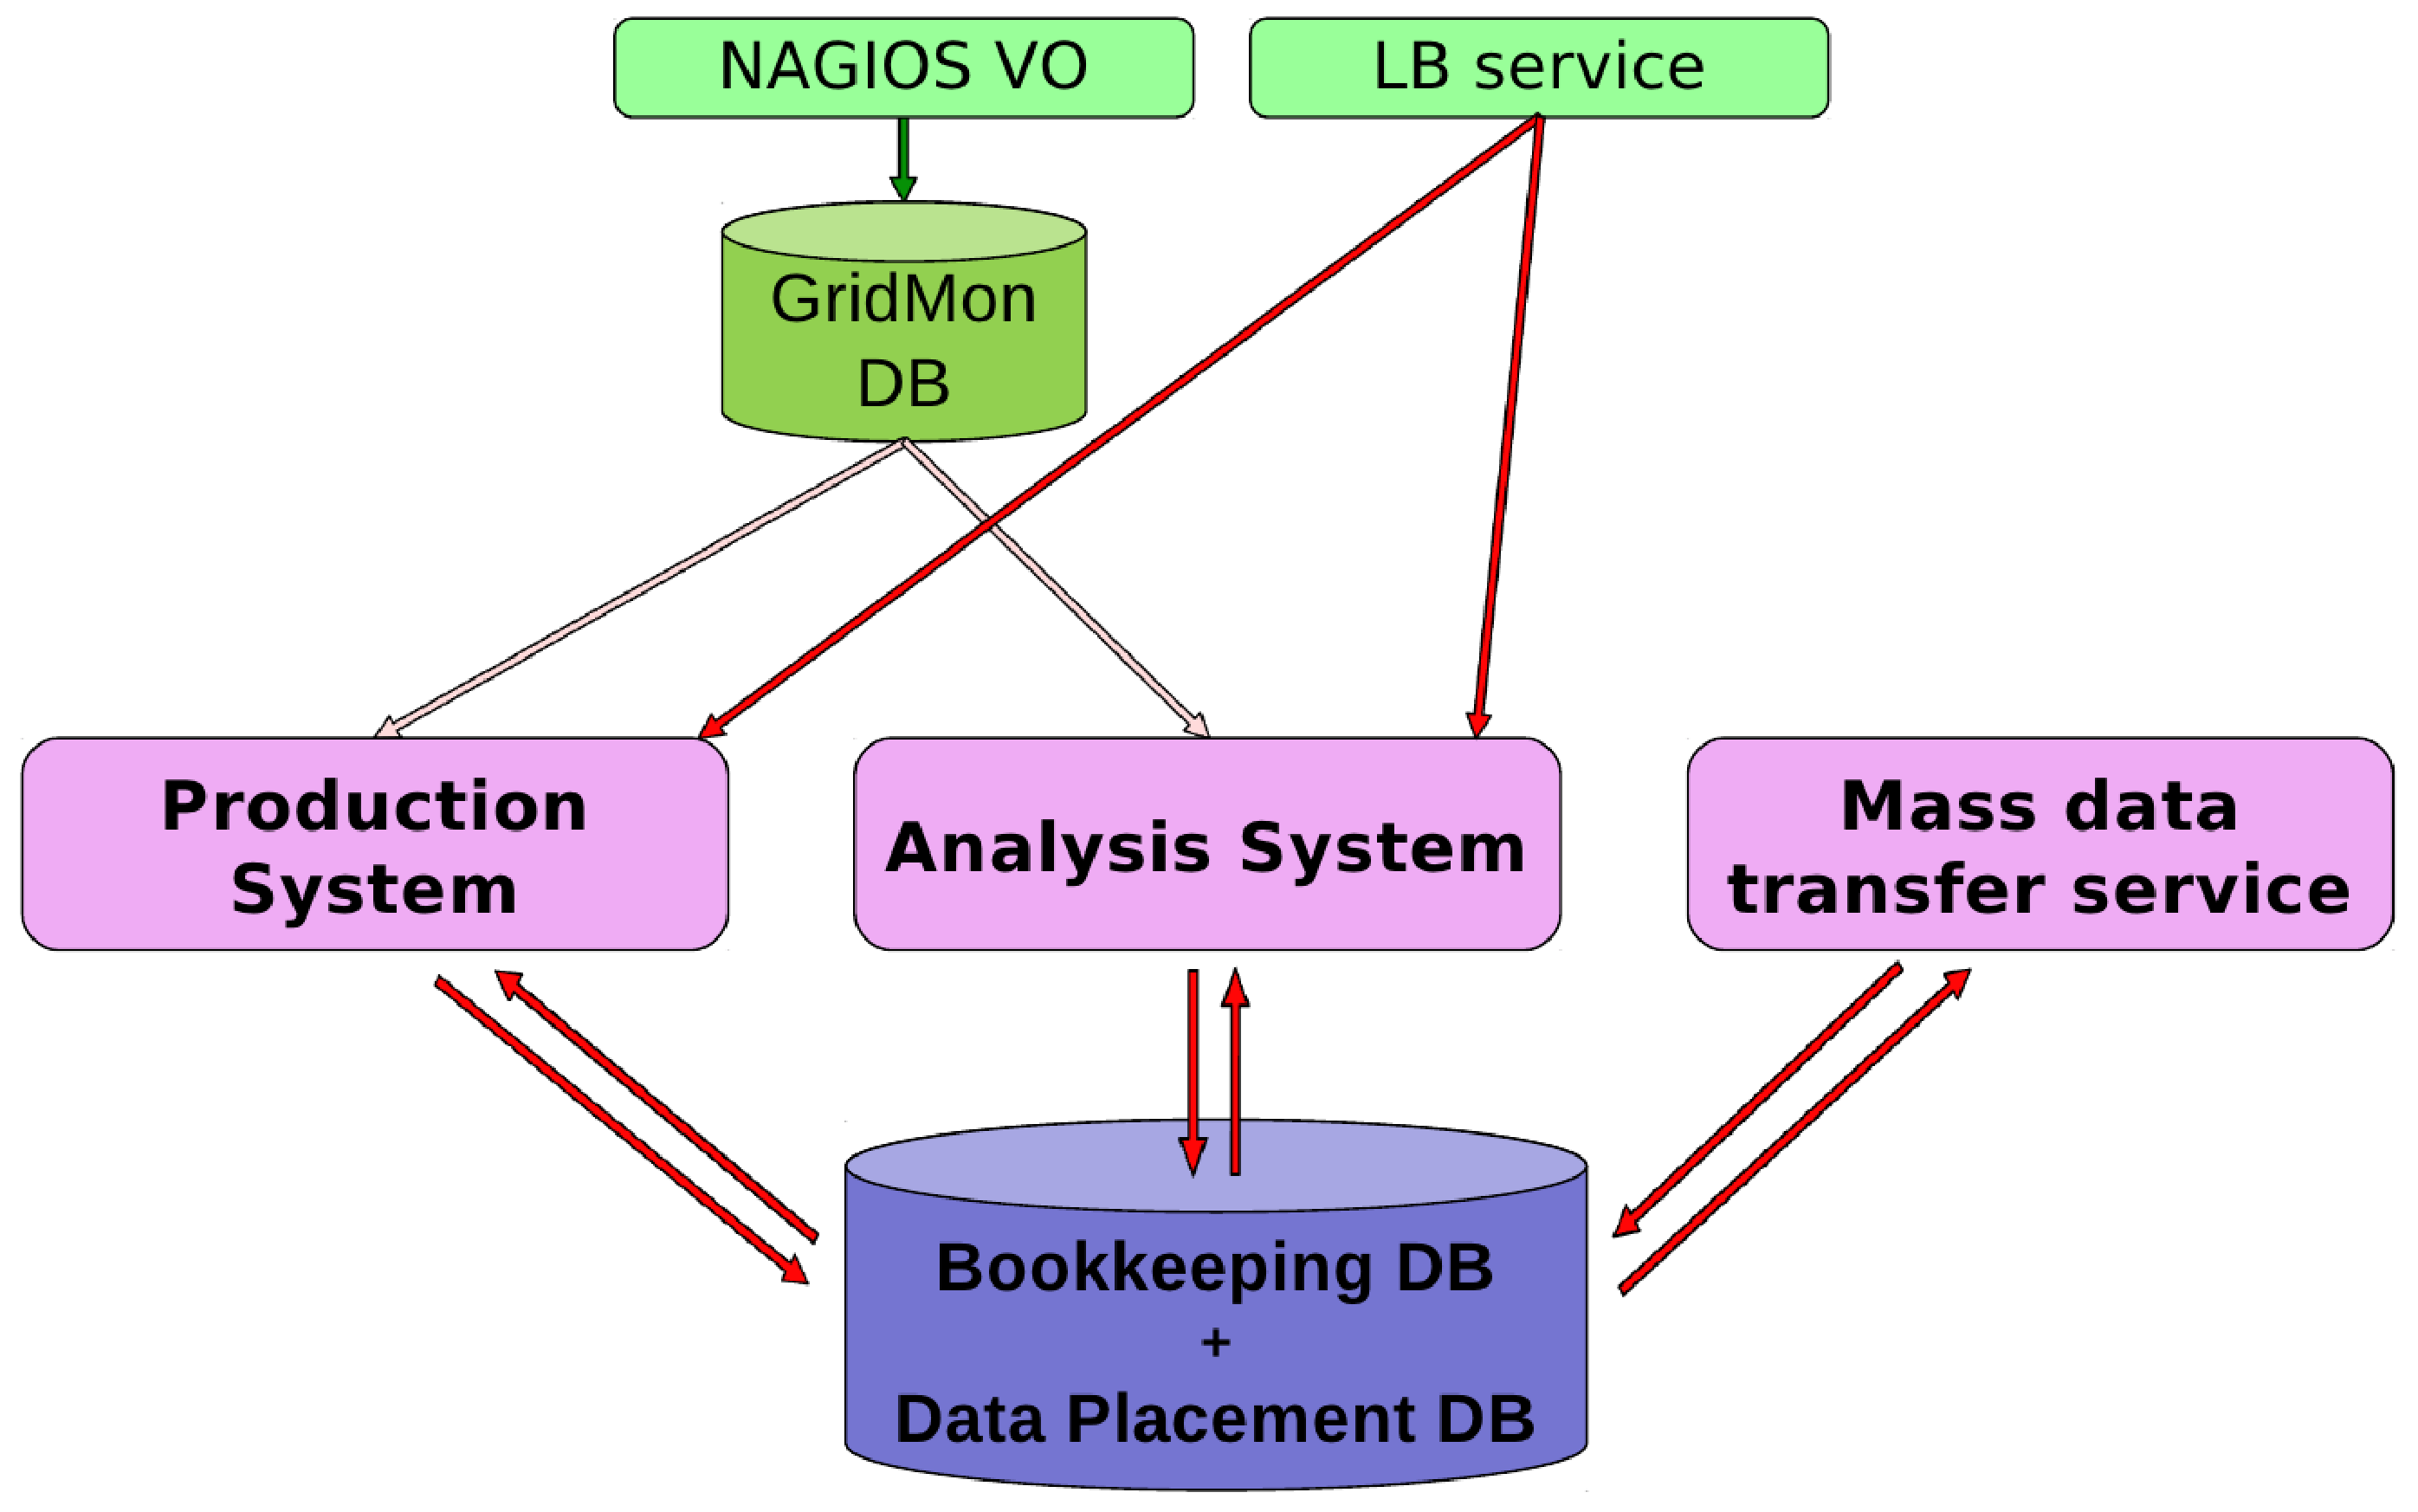
\includegraphics[width=26pc]{img/distributed_system_bird_eye.eps}\hspace{2pc}%
%\caption{\label{fig:distributed_system_bird_eye_view}Distributed System bird's eye view.}
%\end{figure}
 
\section{The Dirac extension} 
% Rafal
DIRAC, born as LHCb MonteCarlo production software, at present time is a complete solution to deploy distributed resources, suitable for large and small communities. DIRAC manage user authentication, authorization and accounting via X509 certificates, applies VO defined scheduling policies, is capable to manage resources made available via different grids, cluster, cloud and desktop computer (via BOINC). Data management capabilities include gLite/EGI storage elements as well DIRAC Storage Elements, LCG File Catalog (LFC) as well DIRAC File Catalog (DFC). The DIRAC webportal offers both user and administrative functionalities. Interfaces can be made using DIRAC API (in python) or a language neutral RESTful interface). DIRAC is widely adopted by large and small communities.\\
DIRAC can be extended to add specific functionalities required by the user. For example in Super$B$\cite{ref:superb_tdr} needs was an interface with a PostgreSQL BookKeeping database and a webportal able to display monitoring data from this database where required. This particular DIRAC extension was named SuperBDIRAC.
%DIRAC Service is a way to export functionalities. 
In SuperBDIRAC a new service, named SBKService, was added to offer an SQLAlchemy layer able to connect DIRAC to a generic SQL DBMS. SBKService maps the bookkeeping (SBK) database using Object Relational Mapping (see section \ref{sec:db}). 
Webportal extension is designed to create and manage simulations, monitoring related jobs and sites. Integration of new functionalities in webportal permits to use only one interface to manage and monitor the entire stack of simulation related tasks.

\section{Bookkeeping DB}
\label{sec:sbk}

\subsection{Description}
A BookKeeping database, named SBK (Super$B$ BookKeeping), have been developed to manage metadata associated with data files. The same database stores information about simulations, executed jobs and output data, site availability in terms of installed and supported software.\\
SBK is used also to schedule jobs submission in order to complete simulations.
Database is modeled to fulfill general requirements of a typical simulation production.\\
Entities in SBK are Session, Production and Request (see figure \ref{fig:BK_entities}). Session defines a simulation (eg. FastSim and FullSim): parameters and software for simulation are defined by VO managers. Production is a Session subset that produce all the  needed to simulate a particular scenario (eg. background in detector).\\
Request is a Production subset. The required number of events to complete a Request is defined during its creation. Request completion is monitored via SBK, allowing job re-submission in order to complete it.\\
SBK design uses the relational model, and the current implementation relies on PostgreSQL (version 9.1) RDBMS which is SQL compliant and, exploiting its hstore datatype, allows to solve some major architectural issues concerning the dataset management of physical parameters. Hstore fields play a major role in the database architecture because storing sets of key/value pairs within a single PostgreSQL value is useful in various scenarios, such as rows with many attributes that are rarely examined, or semistructured data. Beside hstore, some other powerful PostgreSQL features have been exploited: its procedural language (PL/pgSQL) and schemas for a better management of user privileges. An extensive use of views and trigger procedures has been done too.

\subsection{Normalization studies}
During the development phase, the SBK database has been continuously analized in order to guarantee its normal form (NF) 1, 2 and 3 compliance. Four hierarchical levels (production, request, submission and ob+log+output+stat) have been identified for fastsim/fullsim to semplify table definitions and relations. In the production version the SBK database is NF1, NF2 and NF3 compliant with exception of hstore fields. A hstore is a string containing key->value couples and for this reason, if splitted into each couple key->value, it's not NF1 compliant. Since hstore fields permit to reduce database complexity and are rarely accessed (~100 updates every 6 months), a trade-off has been accepted keeping hstore columns not normalized.

\subsection{Stress tests}
Extensive stress tests to check PostgrSQL and HTTP REST interface system robustness have been carried out by means of the Tsung tool (http://tsung.erlang-projects.org/). Tsung allows to create virtual machines for testing scalability and performance of IP based client/server applications in order to do load and stress testing of servers. It can be distributed on several client machines and is capable to simulate hundreds of thousands of virtual users concurrently. For the test phase the REST interface has been configured to establish permanent DB
connections to save connection slots. During the stress tests up to 100 users*s$^{-1}$ have been created. Each user has carried out a connection and 8 insert/update operations on a mock-up database which reproduced the real behavior of a production job. Stress test results were good, being the system capable to sustain 10000 DB transactions (1 transaction = 1 connection+8 insert/update) in ~100s
(~900 operations*sec$^{-1}$).

\section{Bookkeeping DB integration}
\label{sec:db}
% Milosz -> SQLAlchemy
% Luca, Christian -> SBK
%- Software layer based on SQLAlchemy\\
%-- advantages using SQLAlchemy: Object relational Mapping, clean code, fast\\
%-- development, change of DB backend\\
%- BK description, highlighting the general purpose characteristics\\
%-- session, request, dataset concept\\
%****************\\
%Considered alternatives: Psycopg and SQLAlchemy\\
%Why SQLAlchemy?\\
%Powerful object-relational mapping\\
%Elegant, easy to write and read code\\
%Works with wide variety of database backends\\
%*************************\\
MonteCarlo events production needs a method to identify data files and Storage Elements
that holds them. A BookKeeping database have been developed to manage metadata associated with
data files. The same database stores information about simulations, executed jobs and output data, site availability
in terms of installed and supported software.
BookKeeping database is used also to schedule jobs submisison in order to complete simulations.
Database, named SBK (Super$B$ BookKeeping) is modeled to fulfill general requirements of a typical simulation production.
Entities in SBK are Session, Production and Request (see figure \ref{fig:BK_entities}). Session defines a simulation (eg. FastSim and FullSim): parameters and software for simulation are defined by VO managers. Production is a Session subset that produce all the  needed to simulate a particular scenario (eg. background in detector).
Request is a Production subset. The required number of events to complete a Request is defined during its creation.
Final step is submission of jobs needed to complete a Request. Request completion is monitored via SBK, allowing job re-submission in order to complete it. SBK design uses the relational model, and the current implementation uses a centralized PostgreSQL RDBMS.\\
SBK integration in DIRAC is based on SQLAlchemy. SQLAlchemy uses Object Relational Mapper paradigm: database entities are mapped as python objects. SQLAlchemy adoption simplify code writing, reading and documenting\footnote{SQLAlchemy provides an abstraction layer capable to manage in a trasparent way a wide variety of database backends, giving freedom to change it without needs to re-write code.}. 

\begin{figure}[h]
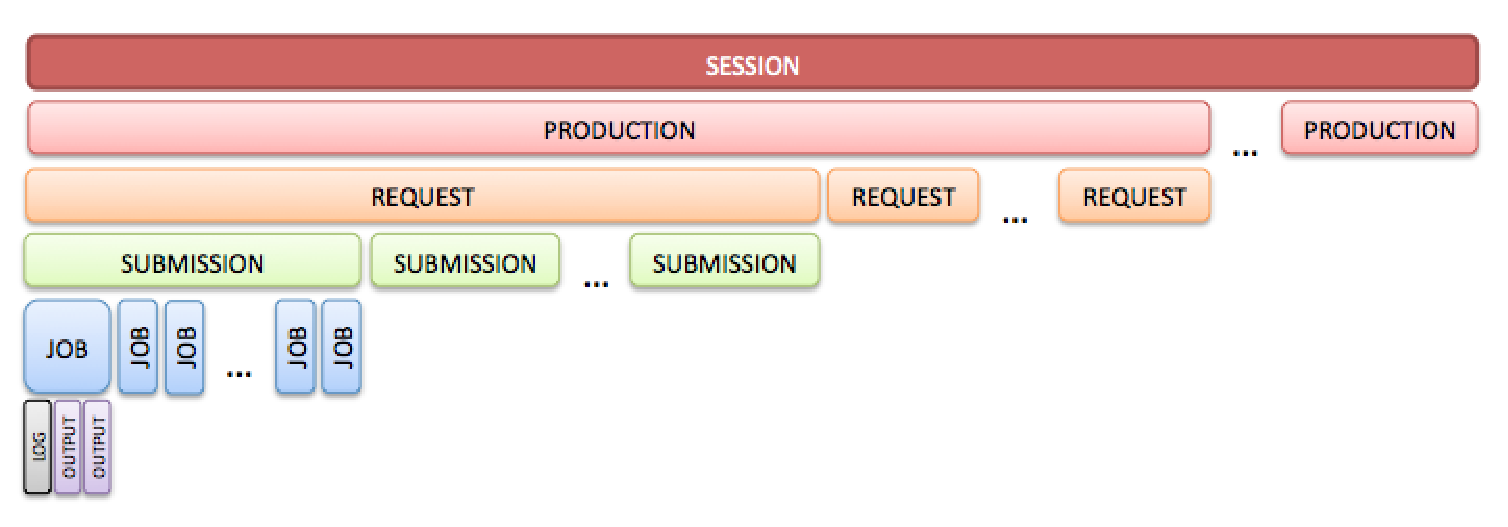
\includegraphics[width=26pc]{img/BK_entities.eps}\hspace{2pc}%
\caption{\label{fig:BK_entities}Entities in BookKeeping database.}
\end{figure}

\begin{figure}[h]
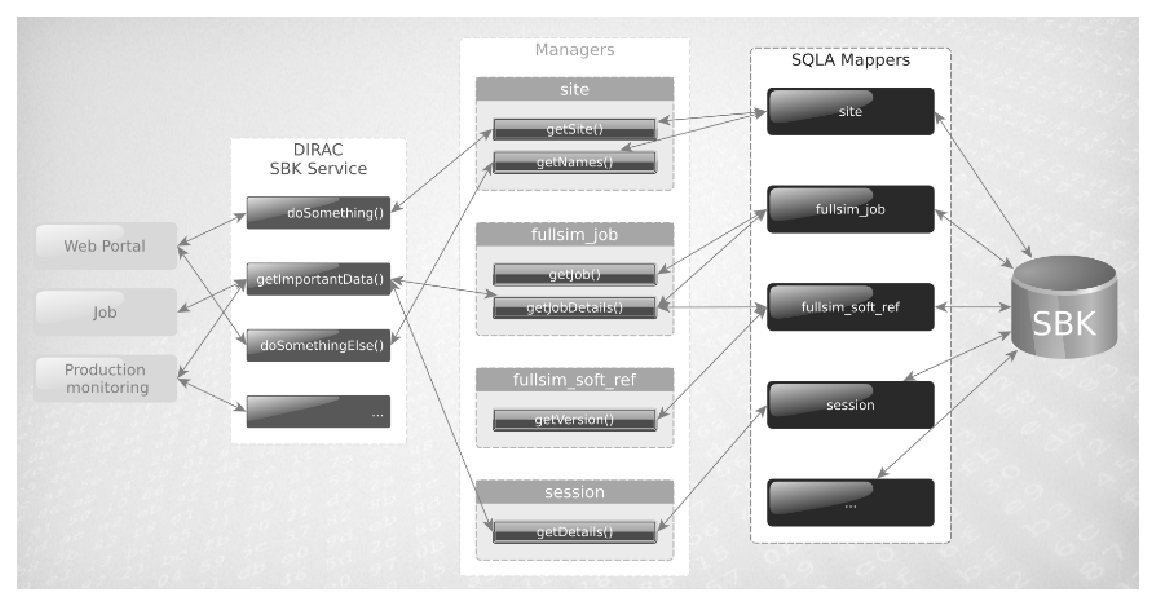
\includegraphics[width=26pc]{img/SBKService.eps}\hspace{2pc}%
\caption{\label{fig:SBKService}SBKService schema.}
\end{figure}
 
\section{Job wrapper component}
\label{sec:severus}

Job wrapper named Severus takes care of main operations of the simulation job:
\begin{itemize}
\item copy software to WN
\item copy input files to WN
\item copy output files in SE and register them in LFC
\item copy log in SE and bookkeping DB
\item update job status in bookkeeping DB
\end{itemize}

\begin{figure}[h]
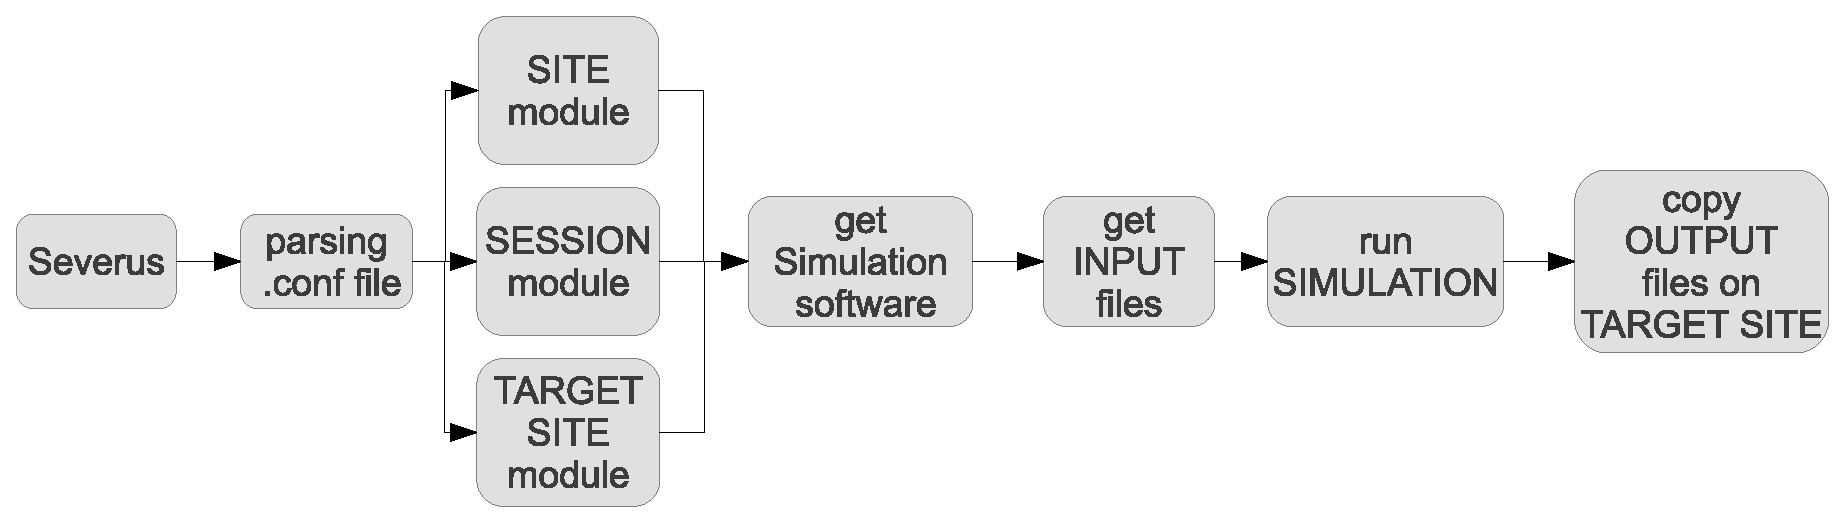
\includegraphics[width=26pc]{img/severus_workflow.eps}\hspace{2pc}%
\caption{\label{fig:severus_workflow}Severus workflow.}
\end{figure}

Access type (lcg or direct) from the worker node to the site SE is automatically recognized and implemented using lcg utils.
A module for each session takes care of properly setting environment variables according to simulation (aka session).
A configuration file customizes its behavior at execution time.
Configuration file has several sections:
\begin{itemize}
\item OPTIONS: general parameters
\item SOFTWARE: info about the executable
\item REST: info about the REST interface to be used for communications with DB
\item SITE: info about the submission site where the job will be runnign. A moduile for eache site is loaded
\item TARGETSITE:  info about site where replicas of output files must be written
\item INPUT: info about the job input files
\item OUTPUT: info for stage-out phase
\item EXPORT VARS: list of envvars to be exported on the WN
\item SESSION\_NAME: key-value pairs for simulation parameters, for the specified session
\end{itemize}
 
\section{Simulation production use case: the SuperB experience}
% Bruno
Simulation Production is designed to manage huge MonteCarlo productions.
A webportal, named WebUI\cite{ref:webui}, is available to manage the entire stack of operations related to this use case: user management, definition of new "Sessions", "Productions" and "Request", job submission and monitoring, sites management for productions. 
Production manager users can add and delete sites, add and delete CEs and SEs, set a site as enabled/disabled and supported/unsopported for a given session, manage "Sessions", "Productions" and "Request". These actions involve only BookKeeping database, building up automatically required tables.
Shifter users can submit and monitor jobs for a given Request. Job submission in WebUI is performed via Ganga\cite{ref:ganga}, while configurations files for submission are generated by WebUI itself taking data from SBK. Ganga submit jobs to grid via WMS using standard gLite commands. Job execution on WNs is driven by Severus (see section \ref{sec:severus}), while job status updates in SBK is performed via REST interface. Stagein and Stageout as well as LFC registration of output files is performed even by Severus. See figure \ref{fig:simulation_production_workflow} for Simulation Production workflow.\\

SuperBDIRAC goal was the porting of the WebUI functionalities in DIRAC to manage jobs and their submission directly from DIRAC and exploite all the funcionalities available in DIRAC: ie. Grid computing resources can be used via WMS or direct submission to CREAM CEs, computer clusters can be accessed via ssh connections, Cloud resources are available via VMDIRAC module, even desktop computers can be used via Boinc. User authentication via X509 certificates and authorization VOMS-role based are builtin in DIRAC.
SuperBDIRAC enhance DIRAC integrating the generic bookkeeping database SBK via SQLAlchemy.
DIRAC webportal is extended in order to provide an interface for Production manager actions as well as shifter tasks.
At present time not all WebUI functionalities are yet ported in SuperBDIRAC, but site and job monitoring from SBK are available.
In section \ref{sec:test} are reported results of first SuperBDIRAC functionality test.

%- general description: workflow, Dirac portal design\\
%- past experience: the webui project\\
%-- Session definition interface --> DB dynamic build up\\

\begin{figure}[h]
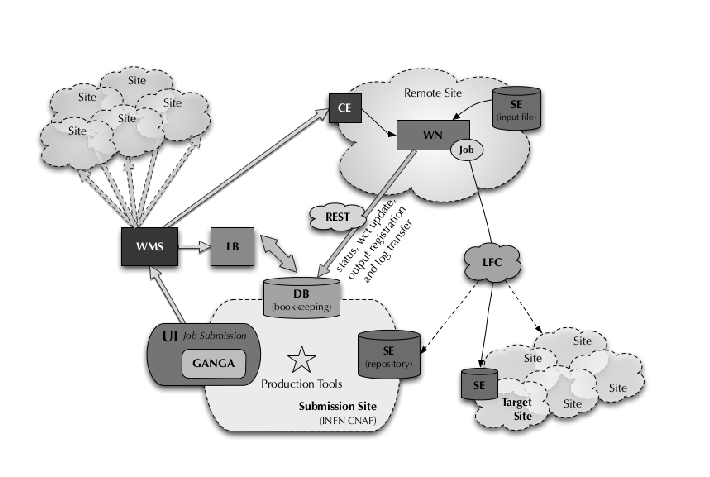
\includegraphics[width=26pc]{img/simulation_production_system_workflow.eps}\hspace{2pc}%
\caption{\label{fig:simulation_production_workflow}Simulation Production workflow.}
\end{figure}
 
\begin{figure}[h]
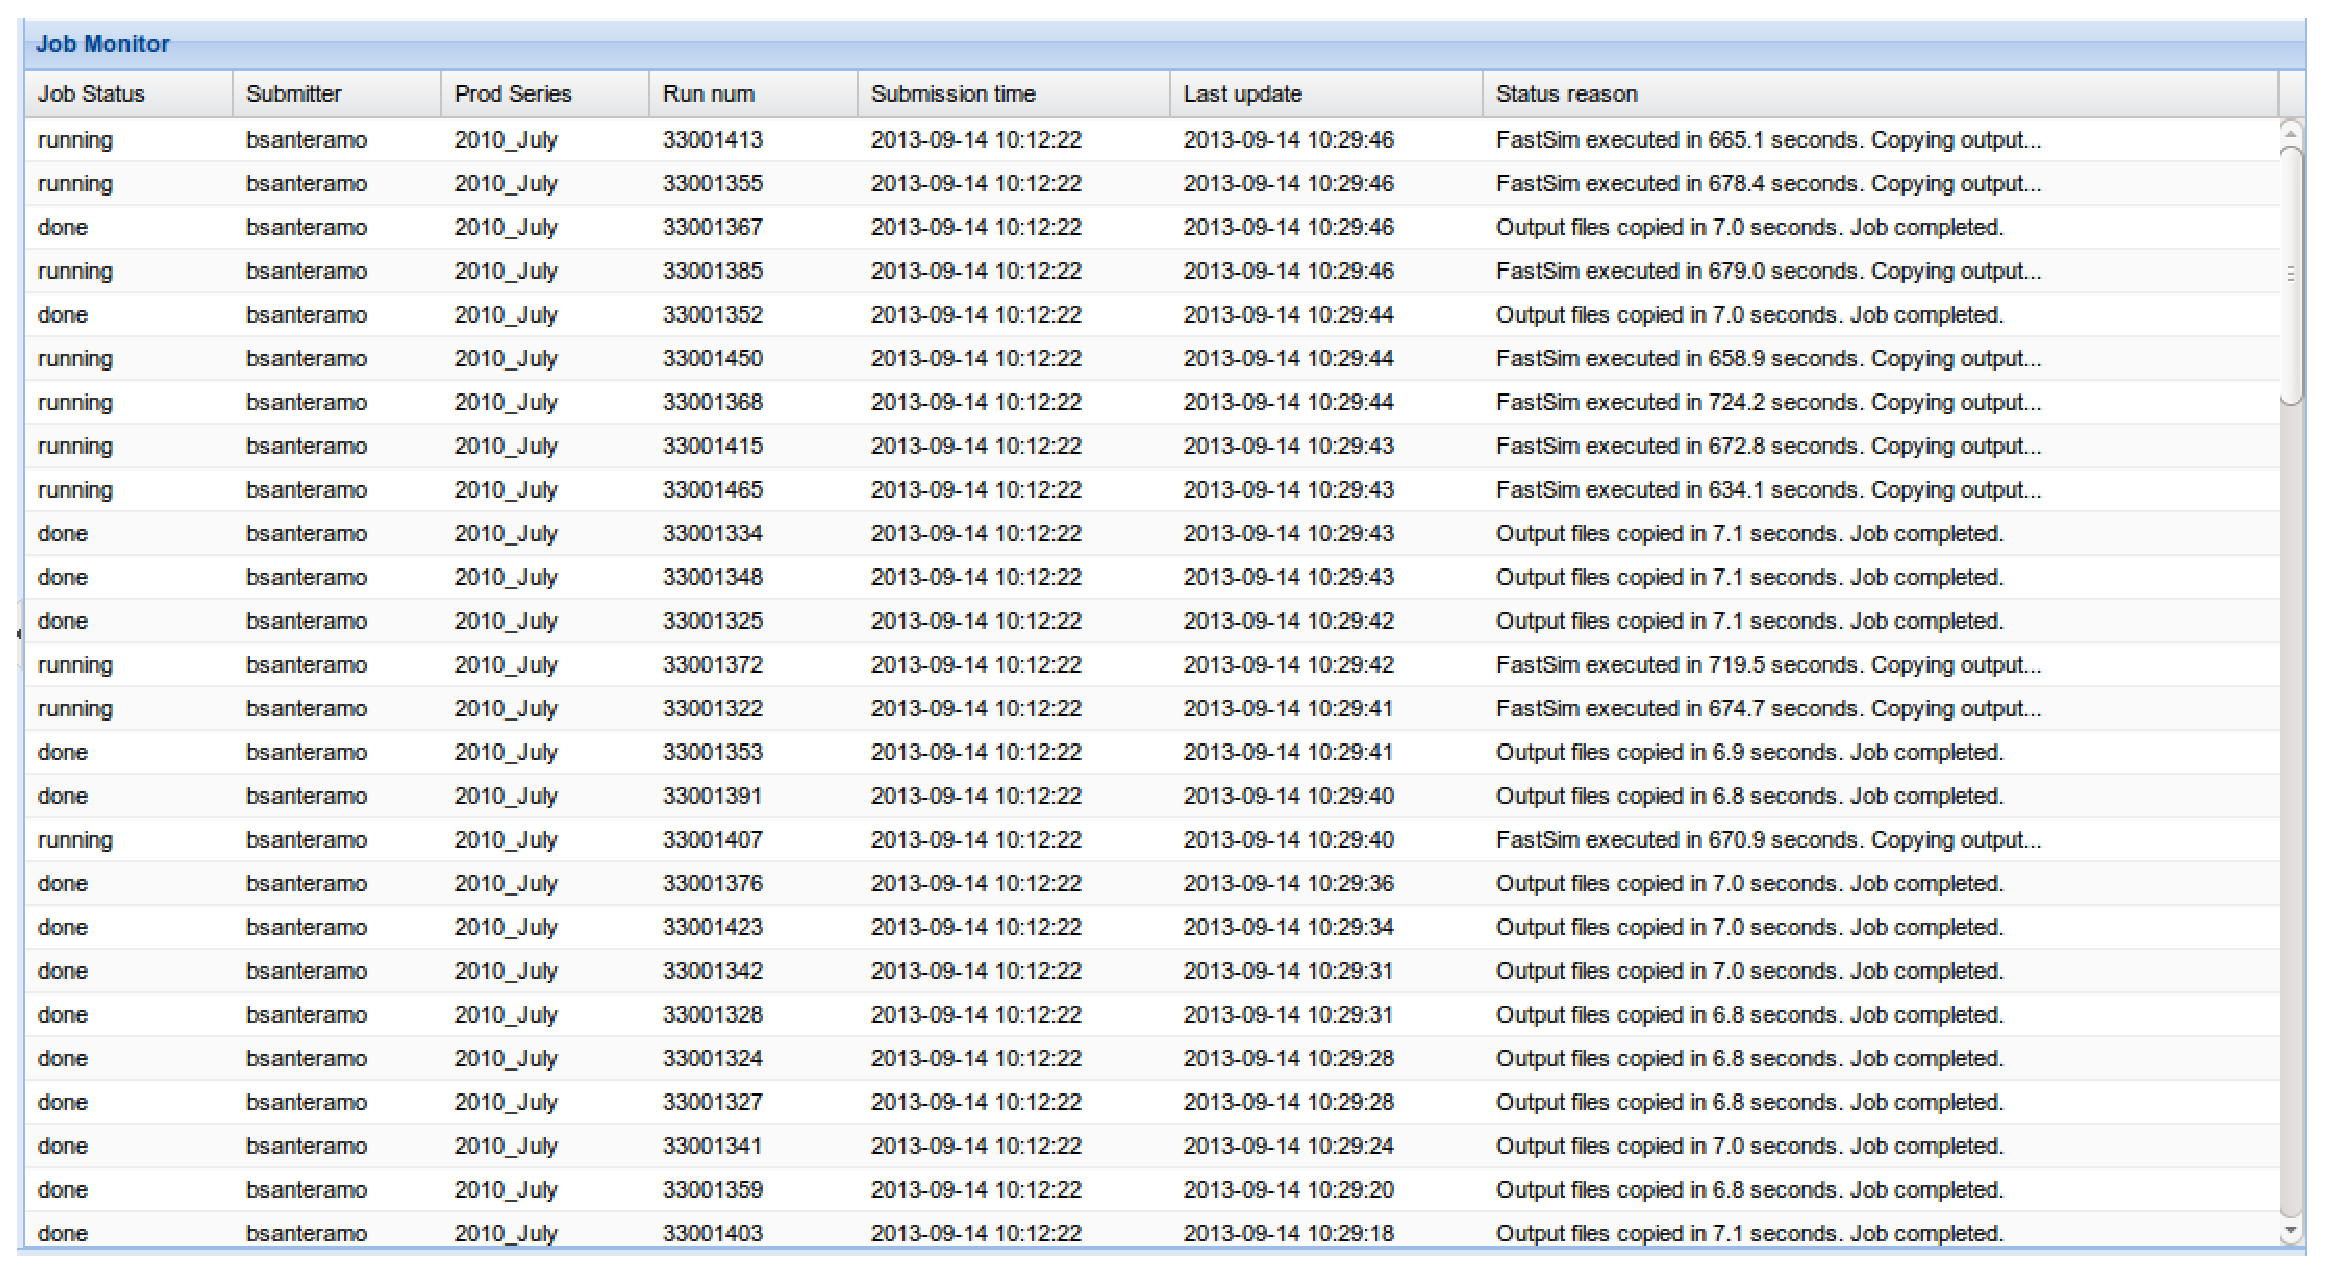
\includegraphics[width=26pc]{img/SuperBDIRAC_monitoring.eps}\hspace{2pc}%
\caption{\label{fig:superbdirac_monitoring}Monitoring job data from SBK in DIRAC.}
\end{figure}

\section{Functionality Test}
\label{sec:test}
% Bruno
A functionality test was performed to demonstrate the capability of SuperBDIRAC to integrate the monitoring of a bookkeeping database in DIRAC webportal.
\subsection{Goal description}
DIRAC capabilities and performance as job management tool are well documented (insert some reference). Super$B$ distributed simulation stack (WebUI + SBK + Severus) was successfully used in 3 simulation campaigns (ask to Armando for confirmation and references).\\
Functionality Test objective is to demonstrate that SuperBDIRAC is capable of substituting WebUI as monitoring tool for job submission and showing data from a bookkeeping database. Test "Q-factor" is the exact correspondence of information as stored in SBK and displayed in SuperBDIRAC, like in WebUI monitoring page. Correct execution of simulation jobs is not important as long as the bookkeping information is properly managed.

\subsection{Testbed description}

\begin{figure}[h]
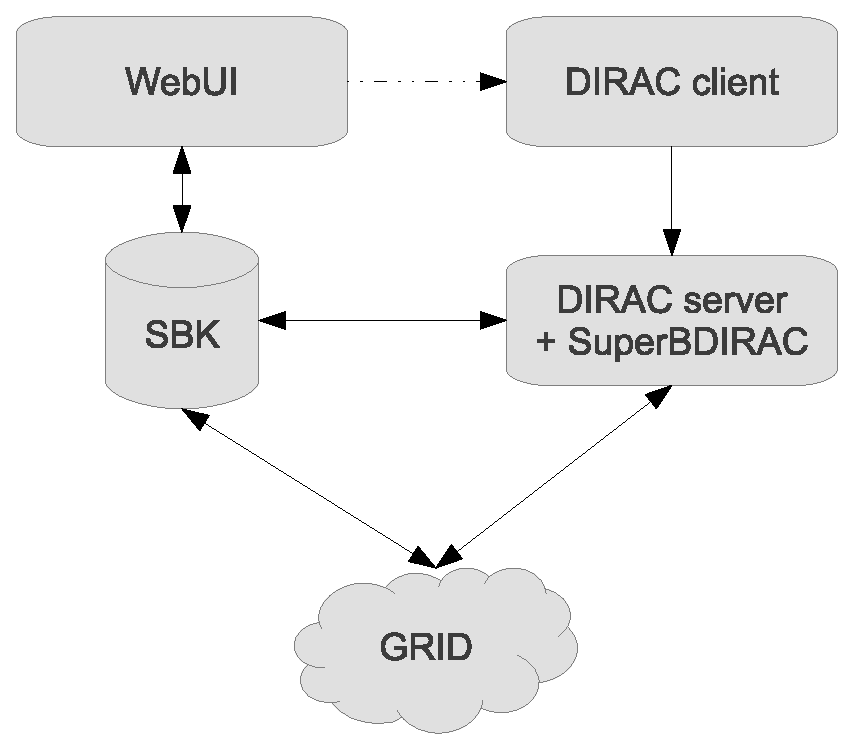
\includegraphics[width=14pc]{img/testbed.eps}\hspace{2pc}%
\begin{minipage}[b]{14pc}\caption{\label{label}Testbed schema.}
\end{minipage}
\end{figure}

At present time, not all WebUI functionalities are implemented in SUperBDIRAC, in particular "Submission" job for a given "Request".
Therefore the following procedure was followed to perform this test. FastSim job submission is created via WebUI interface. Once submission is created, a set of scripts and configuration files are created whose path is shown by WebUI interface. In particular the php submission script, generated by WebUI, is made of an array with all relevant parameters and UI commands needed to submit jobs in grid via standard glite commands.
Since WebUI is still linked with SBK, its portal could be used as well as monitoring portal, useful for a check-cross between info displayed in SBK, WebUI and SuperBDIRAC.\\

The php submission script is parsed by a python script (mc\_production.py), in particular the params array, in order to retrieve all needed paramenters to properly submit jobs via DIRAC: production series, session name, min and max runnumber, configuration files location, physical parameters, events to simulate. Once taken all these parameters, mc\_production.py uses DIRAC API to prepare and submit jobs via DIRAC client.

DIRAC server receive jobs from DIRAC client, than starts the normal workflow for job management in DIRAC: scheduling, pilot submission, payload retrieval and execution, stageout. Since DIRAC server is equipped with SuperBDIRAC, even bookkeeping monitoring is performed by this component.\\

In SBK the job submission insertion is performed by WebUI, while later info are updated by Severus script executed with every submitted job. Severus interact with SBK via REST interface, while WebUI and SuperBDIRAC have direct access to SBK since they are in the same LAN area (ask to Armando for confirmation).\\

Jobs were submitted via grid by DIRAC server. Submission was performed using WMS instead of using direct submission to CREAM CE.\\

Submission site was INFN-T1, which ensured CPU time to execute latest simulations related to Super$B$ once the experiment closure.

\subsection{Test description}

Every job simulated 3000 events: this value is set to have an execution time quite longer than 10 minutes.
Physical parameters are the same of other official productions.
3 main bunch submission of 400 jobs were performed at INFN-T1 to obtain a total of 1200 simulation jobs.
Status in SBK were "prepared", "running" and "done".
In addition, 2 bunch submission of 10 jobs were performed, again at INFN-T1, to force some failure messages in SBK and catch it even in SuperBDIRAC monitoring. First failure sample was obtained setting a not-existing site as destination for stageout: error was detected during preliminary check, so status in SBK were "prepared" and "failed". In second failure sample, jobs were submitted using a proxy without Role=ProductionManager, so error occurred in stageout phase: status in SBK were "prepared", "running" and "failed". In summary, 1220 jobs were submitted for test.\\

During the test execution, several screenshots of WebUI and SuperBDIRAC monitoring were saved, in addition to SBK data screenshots.

\subsection{Results and conclusions}

For each tests, all jobs were submitted at same time. Job execution depends on queue occupancy. Since we were interested in bookkeeping database status updates and not in measuring DIRAC performance in job execution, no dedicated CPU slots were asked for. While failing jobs were all executed simultaneously (10 dedicated CPU were always available for Super$B$ at INFN-T1), for 400 jobs tests simulation execution was spread on a greater time interval (see table \ref{tab:execution_time}).

\begin{table}[h]
\caption{
  \label{tab:execution_time}
  Execution time calculated as difference between Submission time and End Time in DIRAC scheduling system.
}
\begin{center}
\begin{tabular}{lrrr}
\br
test & mean time (sec) & min time (sec) & max time (sec)\\
\mr
good-1 & 2203,66 & 859,00 & 5048,00\\
good-2 & 1102,92 & 832,00 & 2597,00\\
good-3 & 1188,62 & 849,00 & 4716,00\\
failure-1 & 165,10 & 161,00 & 172,00\\
failure-2 & 901,50 & 874,00 & 935,00\\
\br
\end{tabular}
\end{center}
\end{table}

Mean and max time could be interesting for performance measurements, but for this functionality test min time must be considered since it's related to execution time of job ran once submitted. First 3 good test have similar min time, compatible with estimated 13 minutes for simulation. For failure test, in first case the low min time is due to forced error in preliminary check phase (jobs fail without executing simulation code), in second case jobs execute simulation code but fail trying stageout (due to wrong Role-based permission in writing INFN-T1 storage area), so min time is longer as expected.

\begin{table}[h]
\caption{\label{tab:status_update}Job status in SBK, WebUI and SuperBDIRAC.}
\begin{center}
\begin{tabular}{lrlrrrr}
\br
test & jobs & site & SBK status & WebUI status & SuperBDIRAC status & success rate\\
\mr
good-1 & 400 & INFN-T1 & 3 & 3 & 3 & 100\%\\
good-2 & 400 & INFN-T1 & 3 & 3 & 3 & 100\%\\
good-3 & 400 & INFN-T1 & 3 & 3 & 3 & 100\%\\
failure-1 & 10 & INFN-T1 & 2 & 2 & 2 & 100\%\\
failure-2 & 10 & INFN-T1 & 3 & 3 & 3 & 100\%\\
\br
\end{tabular}
\end{center}
\end{table}

BookKeeping database was properly updated for every job in every test. All status change were promptly displayed as well in SuperBDIRAC as in WebUI, without any appreciable delay between two portals. SQLAlchemy didn't introduced any appreciable delay or information loss, at least in this functionality test. 
Table \ref{tab:status_update} reports, for every test, how many status were saved in SBK and displayed in WebUI and SuperBDIRAC. Success rate was established as ratio between status saved in SBK and status displayed in SuperBDIRAC: its value was 100\% in all submissions.
SuperBDIRAC could be considered good enough to integrate in DIRAC the capability of monitoring jobs metadata from a bookkeeping database.

\section{Conclusions}
DIRAC is a mature and stable framework to manage all grid-related tasks, easily adoptable by small as well large VOs.
The Information System is designed to be adapted for a generic huge simulation production.
The Job Wrapper acts as a bridge between simulation jobs and Information System.
We propose SuperBDIRAC as a DIRAC extension capable to satisfy the needs of small and mid size VOs in terms of distributed
resource exploitation.


%% \begin{figure}
%% \begin{center}
%% \includegraphics[width=30pc]{schema.pdf}
%% \caption{Dirac suite design schema}
%% \label{fig:superb_sites}
%% \end{center}
%% \end{figure}


\section*{References}
%%%%%%%%%%%%%%%%%%%%%%%%%%%%%%%%%%%%%%%%%%%

\begin{thebibliography}{30}
%% \bibitem{superb}
%% The Super$B$ Collaboration, \emph{SuperB Progress Report, Detector},
%% \verb"http://arxiv.org/abs/1007.4241v1"

%% \bibitem{ref:miur}
%% \verb"http://www.istruzione.it/web/hub/home"

%% \bibitem{ref:babar}
%% Aubert B et al., 2002 {\it Nucl. Instr. Meth. Phys. Res.}, A 479, 1.

%% \bibitem{ref:belle}
%% The Belle Collaboration 2002 The Belle Detector, {\it Nucl. Instrum. Methods Phys. Res.}, Sect. A 479, 117.

%% \bibitem{atlas}
%% The ATLAS Collaboration, {\it ATLAS Detector and Physics Performance Technical Design
%% Report}, http://atlas.web.cern.ch/Atlas/GROUPS/PHYSICS/TDR/access.html.

%% \bibitem{cms}
%% The CMS Collaboration, {\it CMS Detector Technical Design Report}, http://cmsdoc.cern.ch/cms/cpt/tdr/.

%% \bibitem{ref:chep_dist}
%% Bianchi F, Brown D, Corvo M, Di Simone A, Fella A, Gianoli A, Luppi E, 
%% Morandin M, Paoloni E, Rama M, Tomassetti L 2010 {\it Computing for the Next
%% Generation Flavour Factories}, Proceeding of conference CHEP 2010, Computing for
%% High Energy Physics, Taipei, Taiwan, 18-22 October 2010

%% \bibitem{ref:fast_ieee}
%% Andreassen R et al 2010 {\it FastSim: fast simulation of the SuperB detector},
%% Proceeding of conference IEEE NSS-MIC 2010, Knoxville, TN, USA

%% \bibitem{ref:fast_sim}
%% Di Simone A, Gaponenko I, Manoni E, Perez A, Rama M, Roberts D, 
%% Rotondo M, Simi G, Sokoloff M, Suzuki A, Walsh J 2010 {\it FastSim: fast
%% simulation of the SuperB detector}, Proceeding of conference IEEE NSS-MIC
%% 2010,
%% Knoxville, TN, USA

%% %\bibitem{ref:chep_prod} 
%% %D. Brown, M. Corvo, A. Di Simone, A. Fella, E. Luppi, E. Paoloni, R. Stroili, L.
%% %Tomassetti, \emph{The Distributed Production System of the Super$B$ Project:
%% %Description and Results}. Proceeding of conference CHEP 2010, Computing for High
%% %Energy Physics, Taipei, Taiwan, 18-22 October 2010

%% \bibitem{ref:ieee_prod}
%% Brown D, Corvo M, Di Simone A, Fella A, Luppi E, Paoloni E, Stroili R and Tomassetti L 2010 {\it First Results from the SuperB Simulation Production System}. Proceeding of conference IEEE 2010, NSS-MIC 
%% 2010, Knoxville, TN, USA

%% \bibitem{ref:babar_cm}
%% Bozzi C, Adye T, Andreotti D, Antonioli E, Barlow R, Bense B, Boutigny D, Brew C A J, Colling D, Cowles R D, Elmer P, Feltresi E, Forti A, Grosdidier G, Hasan A,  Lacker H, Luppi E, Martyniak J, McNab A, Petzold A, Smith D A, Sundermann J E and Veronesi P 2003 {\it Using the Grid for the BaBar Experiment}, Nuclear Science Symposium Conference Record, 2003 IEEE, 1626 - 1629 Vol.3

%% %N. Geddes \emph{The BaBar Computing Model}. SLAC-PUB-9964, April 1994

%% \bibitem{egi} 
%% \verb"http://www.egi.eu"

%% \bibitem{osg} 
%% \verb"http://www.opensciencegrid.org"

\bibitem{ref:dirac} 
\verb"http://diracgrid.org"

\bibitem{ref:postgres}
\verb"http://www.postgresql.org/"

\bibitem{ref:sqlalchemy}
\verb"http://www.sqlalchemy.org/"

\bibitem{ref:boinc}
\verb"http://boinc.berkeley.edu/"

\bibitem{ref:superb_tdr}
Super$B$ Technical Design Report, \verb"http://arxiv.org/abs/1306.5655"

%% %\bibitem{ref:nordugrid} 
%% %\verb"http://www.norduGrid.org"

%% \bibitem{ref:westgrid} 
%% \verb"http://www.westgrid.ca"

%% \bibitem{ref:lcg-tdr} 
%% The LCG TDR Editorial Board 2005 {\it LHC Computing Grid}, Technical Design
%% Report LCG-TDR-001 CERN-LHCC-2005-024

\bibitem{ref:ganga}
\verb"http://ganga.web.cern.ch/ganga"

%% \bibitem{ref:wms}
%% \verb"http://glite.web.cern.ch/glite"

%% \bibitem{ref:voms}
%% \verb"http://hep-project-grid-scg.web.cern.ch/hep-project-grid-scg/voms.html"

%% \bibitem{ref:lfc}
%% \verb"https://twiki.cern.ch/twiki/bin/view/LCG/LfcAdminGuide"

%% \bibitem{lcg}
%% \verb"http://lcg.web.cern.ch/LCG"

%% \bibitem{ref:srm}
%% \verb"http://sdm.lbl.gov/srm-wg/doc/SRM.v2.2.html"

%% \bibitem{ref:storm}
%% Corso A et al. 2006 {\it StoRM, an SRM Implementation for LHC Analysis Farms
%% Computing in High Energy Physics} (CHEP 2006), Mumbai, India, Feb. 13-17

%% \bibitem{ref:dcache}
%% Fuhrmann P and Glzow V, dCache 2006 {\it Storage System for the Future}.
%% New York: Lecture Notes in Computer Science/Springer, vol. 4128, pp.
%% 1106-1113.

%% \bibitem{ref:dpm}
%% \verb"https://twiki.cern.ch/twiki/pub/LCG/DataManagementUsefulPresentations/chep 07\_poster_DPM.ppt"

%% \bibitem{ref:hadoop}
%% \verb"http://hadoop.apache.org/"

\bibitem{ref:rest}
Fielding R T 2000 {\it Architectural Styles and The Design of Network-based
Software Architectures }, PhD Thesis, University of California Irvine

\bibitem{ref:webui}
A.Fella, E.Luppi, L.Tomassetti \emph{A General Purpose Suite for Job Management, Bookkeeping and Grid Submission}. International Journal of Grid Computing \& Applications (IJGCA) Vol.2, No.2, June 2011. DOI: 10.5121/ijgca.2011.2202.

\end{thebibliography}

\end{document}
